%%
% 第二章：Franka 平台系统集成与示教数据采集
%%

\chapter{弗兰卡平台系统集成与示教数据采集}
\label{chap:integration}

本章对应设计任务 T1（弗兰卡实时控制与 LeRobot 接口扩展）与 T2（桌面抓取示教数据采集与 LeRobot v2.1 规范化）。设计目标是使 Franka FR3 机械臂被 LeRobot 框架视为标准机器人，从而可复用社区录制与训练工具链，并在此基础上以桌面抓取为实例完成标准化示教数据采集。

全章按“底层执行—框架抽象—人机接口—数据闭环”的层次展开。第二节给出系统四层架构总图与模块职责概览；第三节阐述实时控制与上下位机通信的设计要点；第四节说明如何将弗兰卡平台纳入 LeRobot 的通用机器人抽象，以及带夹爪复合机器人的建模方式；第五节介绍三维鼠标与同构主从两类遥操作方案，并重点给出两阶段配对标定的数学模型与流程；第六节以自采数据集为实例，展示 LeRobot v2.1 规范下的数据组织、特征模式与质量保障措施。

\section{系统总体架构}
\label{sec:arch}

\subsection{四层架构设计}

本文将机器人数据采集平台划分为四层，如图~\ref{fig:four-layer-arch} 所示。各层职责分明，层间通过明确的协议或接口约定解耦，使得实时控制、机器人抽象、遥操作与数据落盘可以独立开发与调试。

\begin{figure}[htbp]
  \centering
  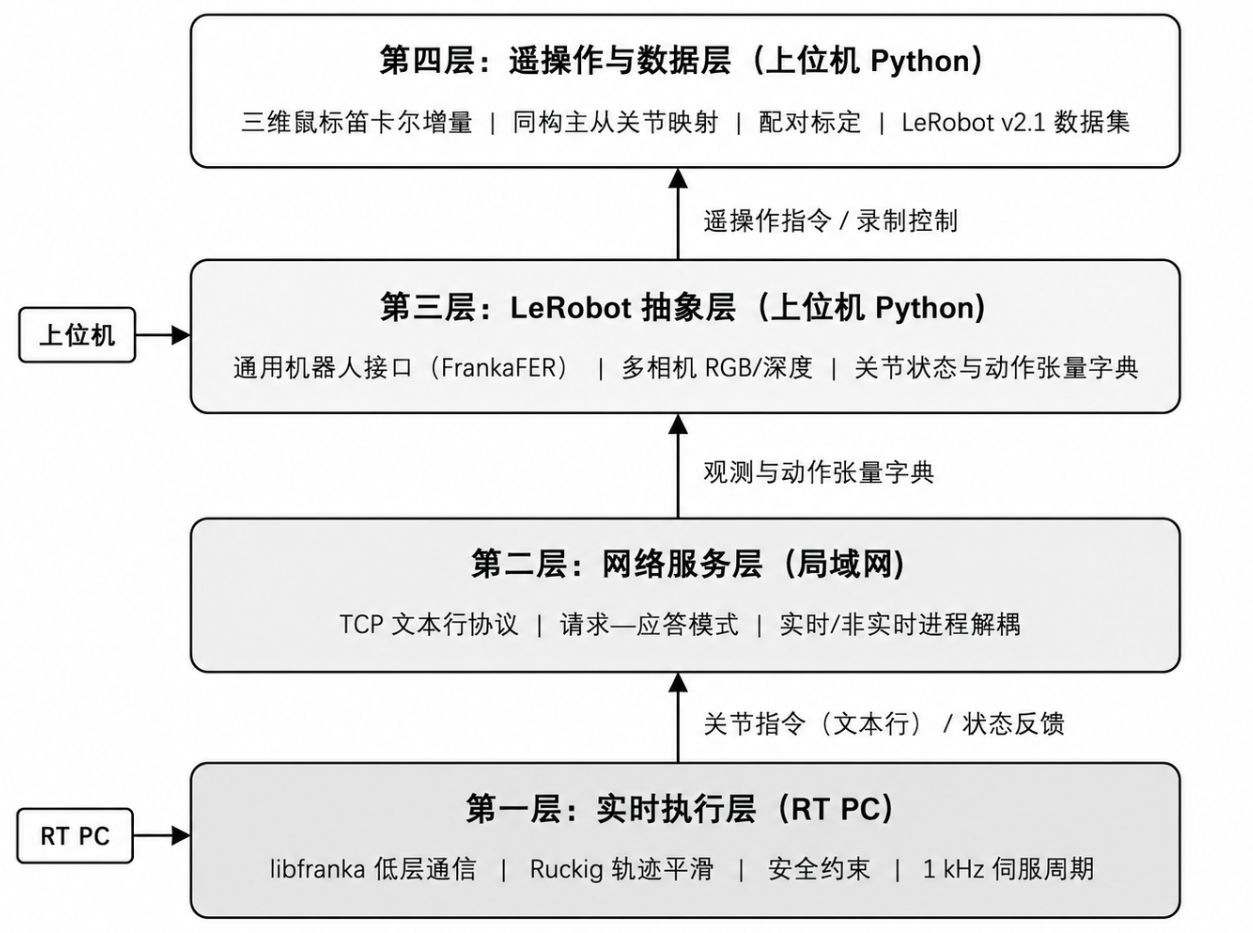
\includegraphics[width=0.92\textwidth]{images/four_layer_arch.png}
  \caption{系统四层架构}
  \label{fig:four-layer-arch}
\end{figure}

第一层为实时执行层，部署于机器人实时控制计算机（RT PC）。该层基于官方 libfranka 库与弗兰卡控制器进行低层通信，并引入 Ruckig 轨迹平滑库对指令做时间参数化，抑制示教或上层指令中的突变，保证 $1\,\mathrm{kHz}$ 伺服周期内的确定性执行。

第二层为网络服务层，通过 TCP 套接字将实时侧与控制计算侧解耦。上位机以文本行协议发送关节目标等指令并接收状态反馈，使实时机仅需维护体量可控的服务端构建产物，上位机则可使用与实验室计算环境一致的 Python 版本与依赖栈。

第三层为 LeRobot 抽象层，在 LeRobot 的 Robot/RobotConfig 约定下实现机器人抽象（FrankaFER 及其夹爪复合配置），将多相机 RGB/深度、关节状态、末端位姿等观测与关节目标等动作统一为张量字典接口，使本平台在框架语义下与社区已有的 Koch、SO-100 等机器人等价。

第四层为遥操作与数据层，实现三维鼠标笛卡尔增量映射与同构主从关节映射两类示教入口，并在 LeRobot 数据集规范下完成多相机—关节状态的时间对齐与字段命名，支撑高质量示教采集。

\subsection{主要软件模块}

表~\ref{tab:module-map} 汇总了平台的主要软件模块及其职责，按所在层次排列。

\begin{table}[htbp]
  \centering
  \small
  \caption{平台主要模块与功能}
  \label{tab:module-map}
  \begin{tabular}{>{\raggedright\arraybackslash}p{3.2cm}>{\raggedright\arraybackslash}p{4.4cm}>{\raggedright\arraybackslash}p{5.6cm}}
    \toprule
    模块 & 所属层次 & 主要职责 \\
    \midrule
    实时控制服务 & 第一层（实时执行） & $1\,\mathrm{kHz}$ 伺服、轨迹平滑、状态回传 \\
    弗兰卡从臂客户端 & 第二、三层 & 套接字通信、观测与动作特征管理、连接生命周期 \\
    臂+夹爪复合配置 & 第三层 & 七轴关节 + 夹爪开合的八维一体化观测与动作 \\
    三维鼠标遥操作 & 第四层 & 鼠标增量—累积位姿—逆运动学—关节目标 \\
    同构主从遥操作 & 第四层 & 主臂读数经缩放偏置映射为从臂关节目标 \\
    配对标定工具 & 第四层（辅助） & 自动解算关节缩放偏置与夹爪量程，输出配置文件 \\
    数据录制管线 & 第四层 & LeRobot v2.1 格式的多相机—关节同步录制与落盘 \\
    \bottomrule
  \end{tabular}
\end{table}

\section{弗兰卡实时控制与底层通信}
\label{sec:franka-server}

\subsection{控制环路与实时性}

弗兰卡机械臂的官方控制接口对实时性有严格要求。本文将低层控制集中于 RT PC 上的 C++ 服务进程，避免在非实时操作系统上与 Python 解释器抢占同一调度上下文，从而降低控制超时风险。服务进程基于 libfranka 读取机器人状态并下发轨迹或目标，同时引入 Ruckig 对指令进行时间参数化和平滑处理，提高执行过程的可重复性与安全性。

\subsection{套接字协议与上下位机分工}

上层 LeRobot 进程不直接调用 libfranka，而是通过 TCP 套接字与实时控制服务进程通信：连接建立后，以换行分隔的文本命令进行请求—应答式交互。该设计的优点在于：首先，上位机可使用与实验室计算环境一致的 Python 版本与依赖栈，便于与 LeRobot、PyTorch 等工具链共存；其次，实时机仅需维护体量可控的服务端构建产物与少量系统依赖，部署边界清晰；最后，便于在局域网内将相机与推理节点与机械臂分机关联，扩展多机协作时的拓扑。

启动数据采集或控制脚本前，须在 RT PC 上先启动实时控制服务并传入机器人 IP，确认健康检查通过后再在上位机侧实例化机器人客户端，以避免“接口已初始化但执行端未就绪”的连接语义错误。

\section{LeRobot 通用机器人接口扩展}
\label{sec:lerobot-robot}

\subsection{框架约定与工厂注册}

LeRobot 将物理平台抽象为 Robot 子类，并通过 RobotConfig 数据类配置（含 type 字段）在工厂函数中派生具体实现。本文在工厂注册中增加了对应系列类型，使标准命令行工具与录制脚本能够以与其他官方机器人相同的方式构造从臂（Follower），无需在外部维护专用启动器。

\subsection{机器人抽象的设计要点}

弗兰卡机器人抽象（FrankaFER）的核心职责包括以下三点。

在连接与生命周期管理方面，配置项中提供实时服务端 IP 与端口；实例化时建立阻塞或非阻塞套接字，并在断开、异常时清理文件描述符，向上层暴露连接状态查询接口，便于录制脚本在断连时安全退出。

在观测特征声明方面，对齐 LeRobot 数据集模式，显式声明各观测键名及类型：七自由度关节位置与速度、末端执行器位姿（以行优先 $4\times4$ 齐次变换矩阵展平为十六维向量）、以及按相机名称组织的 RGB 张量；若启用 RealSense 等相机的深度流，则同步声明对应深度图键名与形状。该声明在录制时用于分配缓冲区与校验字段完备性。

在动作特征与指令下发方面，本文在标准臂控制模式下将动作空间取为七维关节目标位置，键名与 LeRobot 惯用命名一致，便于与后续策略头维匹配。发送时执行”将一行命令编码并写入套接字—读取应答”的同步原语，并对超时与异常进行日志记录与重连策略预留。

上述设计使弗兰卡平台在 LeRobot 语义下与社区已有从臂等价：同一套录制与回放流程可以迁移使用，仅更换配置文件即可。

\subsection{带末端夹爪的复合机器人}

针对桌面抓取任务，机械臂需配合二指夹爪等末端执行器。本文在夹爪复合配置中将臂部与夹爪作为组合实体建模：观测维度在关节与末端位姿基础上扩展夹爪开合相关量；动作维度在七维关节之外增加归一化到 $[0,1]$ 的夹爪指令通道。由此，单条时间步上的“状态—动作”对与单一末端执行器语义一致，降低多设备拼接时的字段分叉与后处理成本。

实物侧采用知行 CTAG2F90C 双指平行夹爪（见图~\ref{fig:zhixing-gripper}），通过法兰与机械臂末端紧固连接；录制与回放时夹爪开合由示教设备或策略输出的标量通道驱动，并在观测状态中保留反馈量以供闭环诊断。

\begin{figure}[htbp]
  \centering
  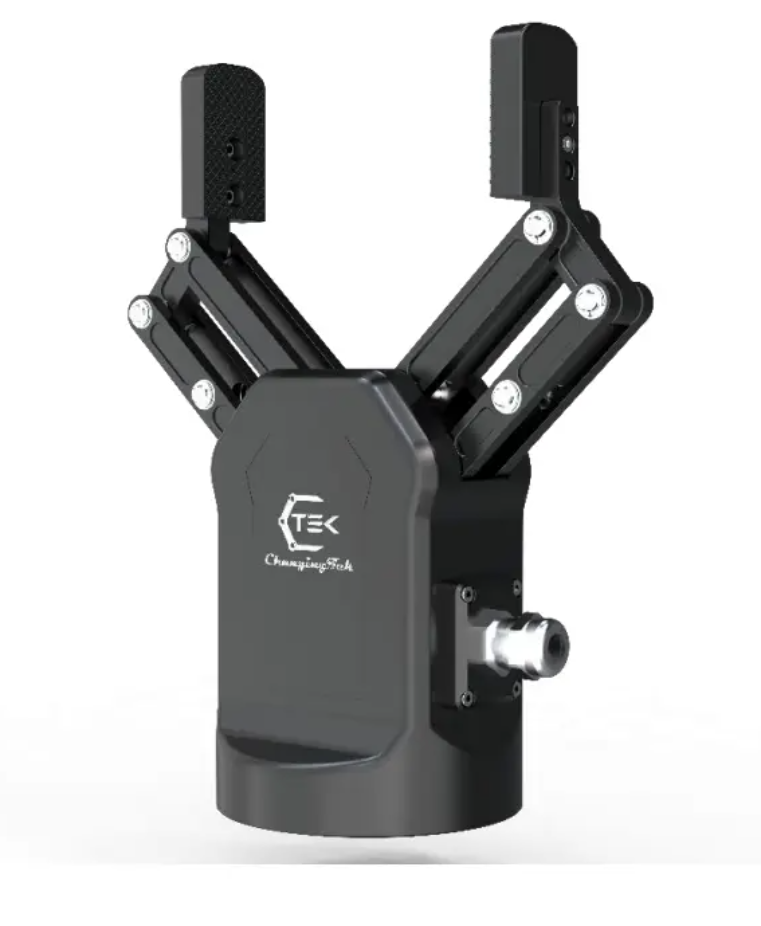
\includegraphics[width=0.32\textwidth]{images/zhixing_gripper.png}
  \caption{知行 CTAG2F90C 双指夹爪安装实物}
  \label{fig:zhixing-gripper}
\end{figure}

\section{遥操作方案设计}
\label{sec:teleoperation}

\subsection{三维鼠标遥操作}
\label{sec:spacemouse}

三维鼠标（SpaceMouse 等六自由度输入设备）能够以较高频率输出线性与角增量的组合，操作者通过推拉、旋转鼠标即可在笛卡尔空间表达末端运动意图。本文在 LeRobot 依赖中利用 pyspacemouse 库读取设备数据，由独立的读取器线程循环采样，将 USB HID 事件转为统一的增量序列号与数值结构，供上层遥操作类消费。

直接将单次增量映射为关节增量容易导致漂移与抖动。本文实现了位姿累积适配器，在笛卡尔空间维护累积位置向量与累积四元数姿态：对每个采样周期，将设备上报的平移增量按可配置标尺缩放，对平移范数与旋转角施加死区，低于阈值的增量置零；合法增量通过四元数乘法累积到当前姿态，且仅在序列号变化时才更新累积状态，避免同一硬件包被重复积分。

设第 $k$ 次有效采样对应的平移增量为 $\Delta \mathbf{p}_k \in \mathbb{R}^3$，姿态增量为单位四元数 $\Delta \mathbf{q}_k$（采用 $(x,y,z,w)$ 约定），则累积位姿更新可写为
\begin{equation}
  \mathbf{p}_{k+1} = \mathbf{p}_k + s \cdot \Delta \mathbf{p}_k ,
  \qquad
  \mathbf{q}_{k+1} = \mathrm{normalize}\bigl(\mathbf{q}_k \otimes \Delta \mathbf{q}_k\bigr),
  \label{eq:spacemouse-pose}
\end{equation}
其中 $s$ 为位置缩放系数，$\otimes$ 表示四元数乘法。死区在平移范数与旋转角上已并入 $\Delta \mathbf{p}_k$、$\Delta \mathbf{q}_k$ 的筛选逻辑。

在获得期望腕部位姿后，需通过逆运动学（IK）解算七轴关节目标。本文复用与 VR 遥操作一致的 IK 求解路径，在 C++ 桥接与 Python 包装之间传递参考关节与目标位姿，对奇异位形与求解失败做异常捕获与日志输出，避免单次 IK 失败中断整条录制会话。

遥操作类继承 LeRobot 的 Teleoperator 基类，实现动作特征声明、连接管理、动作获取等契约：每次获取动作时，将当前鼠标增量经适配器积分后送 IK，输出七维关节目标字典，键名与机器人抽象的动作键一致，从而实现“人通过鼠标在笛卡尔空间表达意图—机器人在关节空间跟随”的闭环。夹爪复合版本在臂部通道上共享同一鼠标读取器，避免对同一 USB 资源双开，夹爪通道则由配置映射为开合标量。

\subsection{同构主从遥操作}
\label{sec:subarm}

相比三维鼠标等笛卡尔空间设备，同构主从允许示教式关节空间映射：操作者拖动与从臂同自由度数的主臂，从臂实时跟踪，可在关节空间完成贴近台面、绕行障碍等细调。主从几何相似时，操作者对主臂的关节角直觉可迁移到对从臂运动的预期，对抓取流水线中的姿态调整往往更直接。

工程上，主臂与从臂的安装轴向、零点与传动比未必一致，因此必须在软件层引入每关节缩放与偏置，并在夹爪通道引入原始量到 $[0,1]$ 的线性标定。若缺少系统化标定，示教轨迹在回放时会出现整体偏转、夹爪“开不满/关不严”等问题，直接污染模仿学习数据集。为此，本文采用如下关节空间映射模型：主臂读出的七关节量经缩放与偏置后作为从臂关节指令。设主臂第 $i$ 关节原始读数为 $\theta^{\mathrm{L}}_i$，经模式函数 $\phi(\cdot)$ 转为主臂侧用于映射的弧度量 $\tilde{q}^{\mathrm{L}}_i$（例如度模式时 $\tilde{q}^{\mathrm{L}}_i=\mathrm{rad}(\theta^{\mathrm{L}}_i)$；规范化模式时 $\phi$ 为恒等映射并保持与运行时一致）。记缩放系数 $\alpha_i$、偏置量 $\beta_i$（单位：rad），则从臂指令为
\begin{equation}
  q^{\mathrm{F}}_i = \alpha_i \, \tilde{q}^{\mathrm{L}}_i + \beta_i ,
  \qquad i=1,\ldots,7.
  \label{eq:subarm-map}
\end{equation}
其中 $\boldsymbol{\alpha}$ 不仅承担比例尺度，更常取 $\pm1$ 以修正轴向反向；$\boldsymbol{\beta}$ 承担零点对齐。同构主从示教的硬件布置实物如图~\ref{fig:franka-subarm-setup} 所示：左侧为 Franka FR3 从臂及末端夹爪，右侧为与从臂同自由度数的主臂；操作者拖动主臂各关节，经缩放与偏置后映射为从臂指令。

\begin{figure}[htbp]
  \centering
  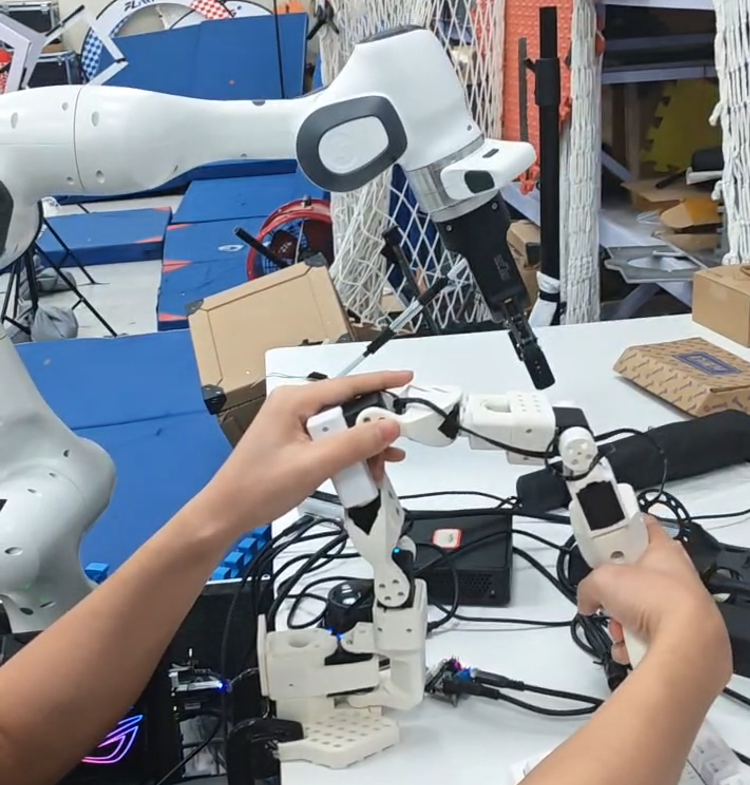
\includegraphics[width=0.5\textwidth]{images/Franka_and_subarm.png}
  \caption{同构主从示教硬件布置}
  \label{fig:franka-subarm-setup}
\end{figure}

基于上述映射模型，为使式~\eqref{eq:subarm-map} 中的 $\boldsymbol{\alpha}$、$\boldsymbol{\beta}$ 及夹爪量程端点可自动解算并版本化，本文设计了两阶段配对标定流程，如图~\ref{fig:calibration-flow} 所示。

\begin{figure}[htbp]
  \centering
  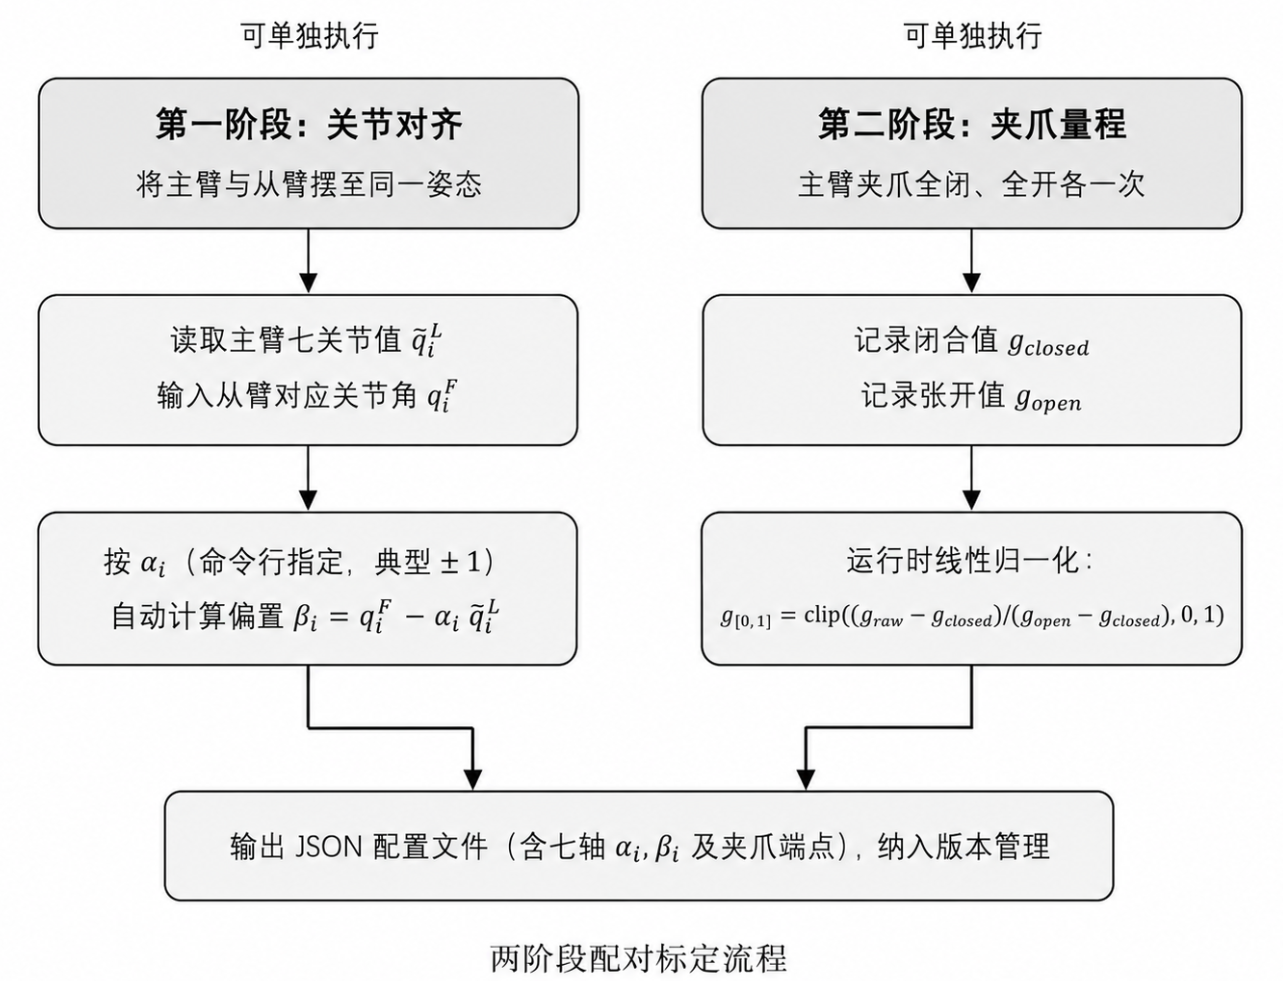
\includegraphics[width=0.92\textwidth]{images/calibration_flow.png}
  \caption{两阶段配对标定流程}
  \label{fig:calibration-flow}
\end{figure}

第一阶段为关节对齐，解算偏置向量。操作者与控制员将主臂与从臂摆到同一物理姿态（建议选用重复性高的初始位姿或示教起点）。脚本通过 SoFranka 读取主臂七关节当前值，按运行时计划使用的度/规范化模式转为 $\tilde{q}^{\mathrm{L}}_i$；同时提示输入从臂该姿态下的七关节角。缩放向量 $\boldsymbol{\alpha}$ 由命令行指定（七个逗号分隔浮点数，典型为 $\pm1$ 组合），偏置自动修正公式为
\begin{equation}
  \beta_i = q^{\mathrm{F}}_i - \alpha_i \, \tilde{q}^{\mathrm{L}}_i ,
  \qquad i=1,\ldots,7,
  \label{eq:subarm-offset}
\end{equation}
其中 $q^{\mathrm{F}}_i$ 为从臂在该对齐姿态的关节弧度。式~\eqref{eq:subarm-offset} 与运行时“先按 $\boldsymbol{\alpha}$ 缩放主臂量、再加 $\boldsymbol{\beta}$”的语义严格一致，从而保证标定与运行时同一解。若主臂工作于度模式而弗兰卡始终以弧度为指令单位，脚本在文档与日志中明确该换算顺序，避免“混用物理单位导致偏置错一个 $\pi$”的常见失误。

第二阶段为夹爪量程，解算开合端点。操作者将主臂夹爪完全闭合与完全张开各一次并在提示时确认；脚本记录两次原始读数，运行时通过线性归一化公式将其映射至 $[0,1]$ 区间，并在开闭读数接近相等等退化情形保留安全截断逻辑。若开闭原始读数方向相反，运行时仍可通过交换端点定义或反向映射保持 $0$ 对应闭合、$1$ 对应张开。

标定脚本支持命令行指定主臂串口、关节读数模式（度制/规范化）、以及单独重标定臂部或夹爪的选项，便于现场迭代。标定结束后以 JSON 统一打印臂部与夹爪字段及注释，可直接进入版本管理，实现“更换主臂/重新固零—重跑脚本—更新配置文件”的闭环。

\subsection{与录制管线的衔接}

两类遥操作方案均实现统一动作获取接口，可与 LeRobot 标准录制流程或自定义循环组合：交替读取机器人观测与遥操作动作，按 LeRobot 数据集模式定义序列化。时间戳对齐上，以机器人状态回执或统一主机时钟为基准，对图像帧与关节指令做最近邻或插值对齐；工程上通过固定控制频率与阻塞读减少抖动，并在元数据中记录相机帧率与伺服周期。

经过配对标定后的主从映射，可显著降低“同一条示教意图”在关节空间的批间方差，有利于小规模高质量轨迹上策略网络的收敛与泛化——该数据规模与后续 $\pi_{0.5}$ 实验章节相对应。

\section{桌面抓取示教数据采集与 LeRobot 数据集规范}
\label{sec:data-collection}

前面各节从工程实现角度完成了机械臂与 LeRobot 的接口打通，并给出了三维鼠标与同构主从两类遥操作方案及其标定流程。本节以实际落地的示教采集流水线为对象，说明采集任务设定、落盘数据如何组织为 LeRobot 官方数据集形态，以及为何该字段编排与多相机布局适合本文的桌面抓取与后续 $\pi_{0.5}$ 类策略训练。

\subsection{采集任务与录制流程}
\label{sec:task-record}

采集任务设定为：“抓取绿色苹果并放置至桌面左上角”。每条示教轨迹的语言指令单独登记在任务元数据中，全库共 30 条轨迹，在统一任务语义下由操作者通过同构主从臂重复示教完成。

数据录制采用双相机布局：第三人称固定相机获取全局场景信息（桌面目标物位置、放置区域、障碍物等），腕部手眼相机提供夹取局部几何（手指—物体相对关系、闭合接触状态等）。两者以统一的 $10\,\mathrm{Hz}$ 帧率同步录制。对于桌面抓取这类以准静态接触与柔顺放置为主的操作，该帧率在保证任务相关运动信息不丢失的前提下，降低了存储与解码开销，并与 LeRobot 训练数据加载器的常见假设兼容。

录制流程的整体数据流如图~\ref{fig:data-collection-flow} 所示。

\begin{figure}[htbp]
  \centering
  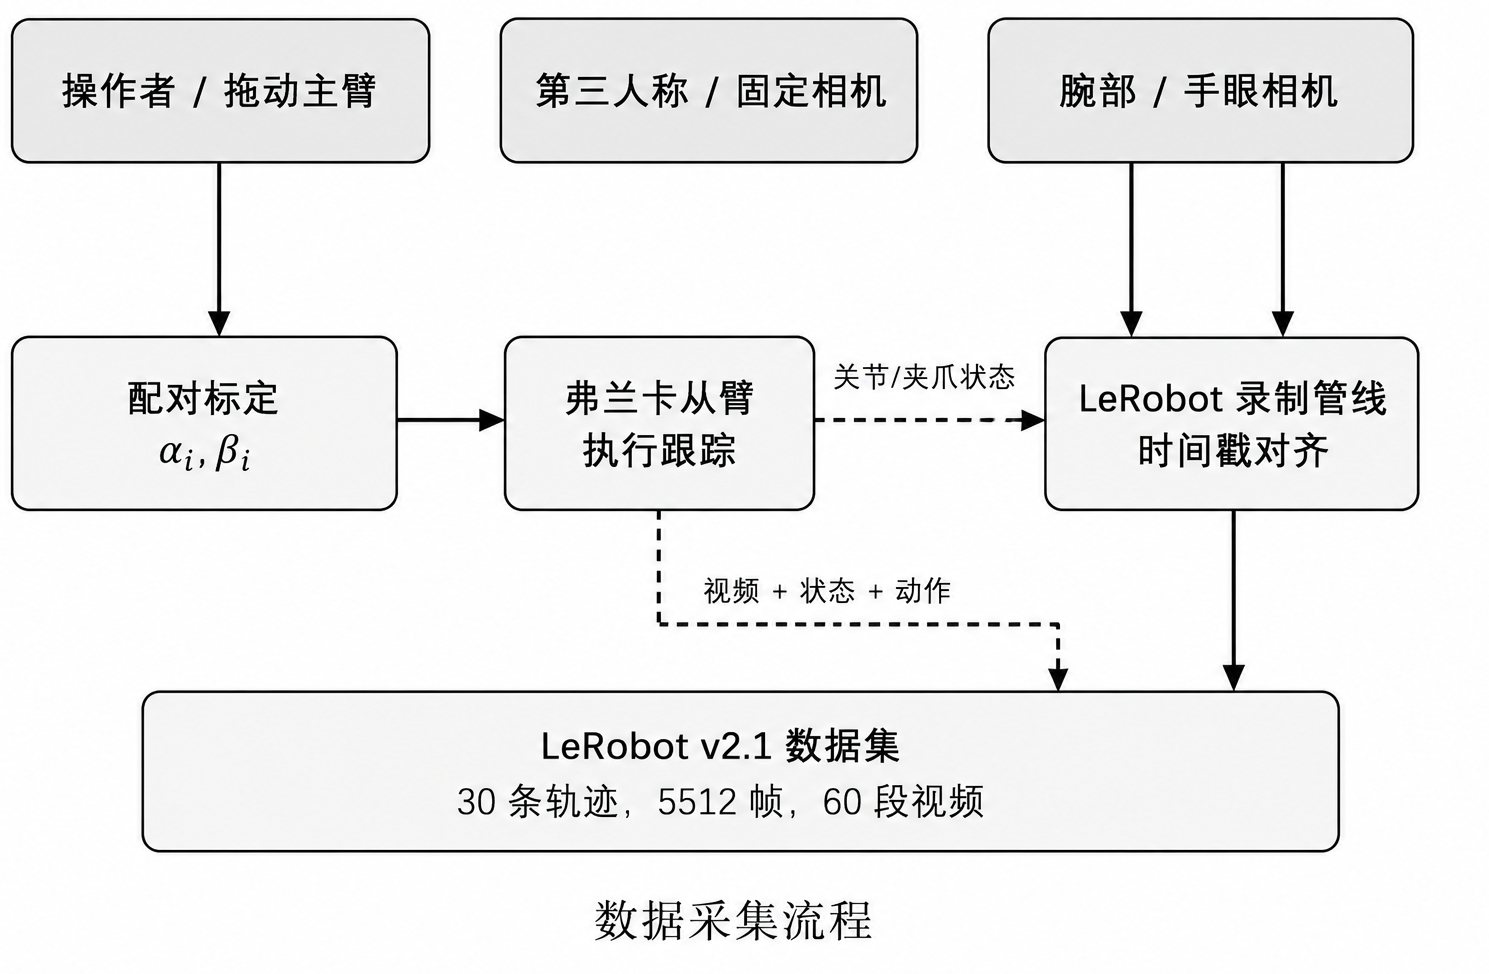
\includegraphics[width=0.92\textwidth]{images/data_collection_flow.png}
  \caption{数据采集流程}
  \label{fig:data-collection-flow}
\end{figure}

\subsection{LeRobot v2.1 数据集组织}

数据集严格遵循 LeRobot v2.1 目录规范，核心由三类路径组成：元数据目录存放全局说明与轨迹列表（机器人类型、总帧数、各字段名称与形状、任务语义与轨迹元信息）；数据目录以列式存储格式（Parquet）按分块存放帧级表格，每文件对应一整条轨迹的时间序列样本；视频目录存放与表格行对齐编码的外挂视频轨道，每个相机、每条轨迹各一条 MP4 视频。

该布局的价值在于：表格存低维时序量（关节角、夹爪开合、末端位姿等），视频存高维图像流，二者通过统一的帧索引与时间戳字段建立一一对应关系；训练代码只需按 LeRobot 的特征声明进行张量拼接，无需定制私有数据加载器。

\subsection{帧级特征模式}
\label{sec:feature-schema}

表~\ref{tab:pick-apple-features} 归纳了数据集中声明的主要特征键。动作空间与关节观测在维数与命名上呈对齐关系：均为八维浮点向量，前七维对应弗兰卡七轴关节位置，第八维为夹爪开合通道。这种“状态—动作同构”的写法是行为克隆与扩散策略类方法的常见输入形式：网络在时刻 $t$ 读取多相机图像与本体状态，预测监督目标为同刻示教者给出的关节—夹爪指令或下一时刻目标。

\begin{table}[htbp]
  \centering
  \small
  \caption{数据集主要帧级特征}
  \label{tab:pick-apple-features}
  \begin{tabular}{>{\raggedright\arraybackslash}p{4.2cm}>{\raggedright\arraybackslash}p{1.4cm}>{\raggedright\arraybackslash}p{2.3cm}>{\raggedright\arraybackslash}p{4.3cm}}
    \toprule
    特征键 & dtype & 形状概要 & 含义（本文设置下） \\
    \midrule
    action & float32 & $8$ & 示教关节目标 + 夹爪指令，用于监督学习 \\
    observation.state & float32 & $8$ & 关节位置与夹爪反馈，构造策略条件 \\
    observation.velocity & float32 & $7$ & 七轴关节角速度，可选辅助信号 \\
    observation.eepose & float32 & $7$ & 末端位姿 $(x,y,z,q_x,q_y,q_z,q_w)$ \\
    \shortstack[l]{observation.images.\\wrist} & 视频 & $720{\times}1280{\times}3$ & 腕部/手眼 RGB，$10\,\mathrm{fps}$ \\
    \shortstack[l]{observation.images.\\third\_person} & 视频 & $720{\times}1280{\times}3$ & 第三人称场景 RGB，$10\,\mathrm{fps}$ \\
    timestamp 等索引字段 & 标量 & $1$ & 帧内时间戳、轨迹/任务编号、全局行号 \\
    \bottomrule
  \end{tabular}
\end{table}

多相机观测分别以腕部与第三人称两个键挂载。二者在物理视角上互补：第三人称摄像机提供桌面上苹果目标物、障碍物与边角放置区域的全景关系，适于粗定位与语义对齐；腕部摄像机则提供抓取对准期所需的局部几何与开合过程中的手指—物体相对关系，对降低从侧面观看时的深度歧义至关重要。分辨率 $1280{\times}720$、采样率与关节序列一致且视频参数在特征信息块中逐项声明（像素格式、是否具有深度、是否含音频等），保证了跨机器解码的可重复性。

低维本体量除关节状态外，另含七维关节速度与七维末端位姿。前者可用于未来引入速度惩罚或对比学习；后者便于在调试阶段与笛卡尔空间示教设备（如三维鼠标路径）进行交叉验证。对于以关节空间监督为主的 $\pi_{0.5}$ 管线，核心训练张量落在多相机图像与动作（及必要的本体状态）之上，其余字段以“可扩展但不扰动训练接口”的方式存在。

\subsection{数据规模与质量保障}
\label{sec:scale-quality}

在规模上，30 条轨迹、合计 5512 帧属于小规模专用数据集，适用于在基础 VLA 模型上进行任务特化微调或概念验证，而不追求覆盖所有桌面扰动。单条轨迹长度在约一百七至一百九十余步之间波动，对应十几秒量级的操作过程，与“抓取—移动—放置”三阶段结构相符。

从数据质量角度，本文在采集端强调三个要点。首先是字段完备性，关键键名符合 LeRobot 约定，减少训练脚本中的硬编码映射。其次是时间一致性，统一 $10\,\mathrm{Hz}$ 与外挂视频，使视觉与关节标签天然对齐。最后是任务语义显式化，自然语言任务写入元数据并在轨迹信息中重复索引，便于多任务扩展或与语言条件策略对接。在此前提下，即使样本量有限，网络仍主要学习桌面绿色苹果抓取并置于桌面左上区域这一窄分布，与后续章节对 $\pi_{0.5}$ 结构的针对性改进及桌面实验评价形成闭环。

